\documentclass[printbox]{BHCexam}
% \documentclass[openright,oneside]{ctexbook}	% 加[draft]选项可不显示图片本体,加快编译,全文完成后再删除

\biaoti{~$2019$~汤家凤考研线性代数强化}
\fubiaoti{邱日笔记}
\usepackage{ctex}
% \usepackage[heading=true]{ctex}

\usepackage{palatino}
\usepackage{siunitx}%输入度数符号需要的单位宏包
\usepackage{tikz}
% \usepackage[fntef]{ctexcap}
\usepackage{enumitem}
\usepackage{amsmath}
\usepackage{cases}
\usepackage[]{titlesec}
\usepackage{comment}%参看宏包说明
\usepackage{bbding}

% \usepackage[center]{titlesec} %其中 center 可使标题居中,还可设为 raggedleft (居左,默认), raggedright (居右)。
% \titleformat{\chapter}{\centering\Huge\bfseries}{第\,\thechapter\,章}{1em}{}
%\CTEXsetup[name={第,章},number={\chinese{chapter}}]{chapter}

\usetikzlibrary{shapes.geometric, arrows}
\tikzstyle{startstop} = [rectangle, rounded corners, minimum width = 1cm, minimum height=0.5cm,text centered, draw = black]
\tikzstyle{io} = [trapezium, trapezium left angle=70, trapezium right angle=110, minimum width=0.5cm, minimum height=0.5cm, text centered, draw=black]
\tikzstyle{process} = [rectangle, minimum width=2cm, minimum height=0.5cm, text centered, draw=black]
\tikzstyle{decision} = [diamond, aspect = 3, text centered, draw=black]
% 箭头形式
\tikzstyle{arrow} = [->,>=latex]
\begin{document}
\AddEnumerateCounter{\chinese}{\chinese}{}

\printanswers % 我要打印答案

% \titleformat{\chapter}{\centering\Huge\bfseries}{第\,\thechapter\,章}{1em}{}
% \titleformat{\section}[block]{\centering\LARGE\bfseries}{第 \arabic{section} 章}{1em}{}
\titleformat{\section}[block]{\centering\LARGE\bfseries}{第 \chinese{section} 章}{1em}{}
\titleformat{\subsection}{\Large}{\chinese{section}. }{1em}{}
% \titleformat{\section}{\Large}{第\chinese{section}节 }{1em}{}
% \titleformat{\subsection}[block]{\Large\bfseries}{ \Roman{subsection}}{1em}{}
% \titleformat{\subsubsection}[block]{\large\bfseries}{\Roman{subsection}-\alph{subsubsection}}{1em}{}
% \titleformat{\paragraph}[block]{\normalsize\bfseries}{[\arabic{paragraph}]}{1em}{}


\maketitle  
% 暂时不搞标题节省时间

%\mininotice

% $\left(                 %左括号
% \begin{array}{ccc}   %该矩阵一共3列,每一列都居中放置
%   a11 & a12 & a13\\  %第一行元素      
%   a21 & a22 & a23\\  %第二行元素
% \end{array}
% \right)$      

\tableofcontents

\clearpage
% \part{部分标题}

% 垃圾


% \chapter{章标题}这一章我们介绍这些内容。

\section{行列式}
\subsection{defs}

\paragraph{1.} 逆序: $i,j \in N , if(i > j)  $
\paragraph{2.}  逆序数 \\
% \begin{enumerate}
  % \item 逆序: $i,j \in N , if(i > j)  $
  % \item 逆序数
  % \item 
  % \paragraph{}
D = $\begin{pmatrix} \begin{matrix} a_{ 11 } & ,... & a_{ 1n } \\ ... & ... & ... \\ a_{ n1 } & ... & a_{ nn } \end{matrix} \end{pmatrix}$=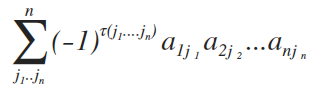
\includegraphics[scale=0.5]{assets/1-1.png}
  % $\begin{pmatrix} \begin{matrix} a_{ 11 } & a_{ 12 } & a_{ 13 } \\ a_{ 21 } & a_{ 22 } & a_{ 23 } \\ a_{ 31 } & a_{ 32 } & a_{ 33 } \end{matrix} \end{pmatrix}$ \\
$$=+a_{11} a_{22} a_{33} -a_{11} a_{23} a_{32} -a_{12} a_{21} a_{33} +a_{12} a_{23} a_{31}
+a_{13} a_{21} a_{32} -a_{13} a_{22} a_{31}
$$ 

  $\tau{(2\;5\;6\;4\; 1\; 2)} = 2+3+3+2$ 
  
    % +a_{11} 
  $\tau{(1 2 3)}=0,\tau{(132)}=1,\tau{(213)}=1,\tau{(231)}=2,\tau{(312)}=2,\tau{321}=3$

  \begin{numcases}{a_{11}}
   a_{22}  \qquad a_{33}\\
   a_{23}  \qquad a_{32}
  \end{numcases}
  \begin{numcases}{a_{12}}
    a_{21}  \qquad a_{33}\\
    a_{23}  \qquad a_{31}
   \end{numcases}
   \begin{numcases}{a_{13}}
    a_{21}  \qquad a_{32}\\
    a_{22}  \qquad a_{31}
   \end{numcases}

   \paragraph{3.}
   \begin{questions}
   \question 已知  ~$f(x)$~ = $\left(                 %左括号
   \begin{array}{ccc}   %该矩阵一共3列,每一列都居中放置
     2x-1 & x+2 & 3\\  %第一行元素      
     -1 & x+4 & 3-2x\\  %第二行元素
     5 & 3x+2 & x+2\\ 
   \end{array}
 \right)$                 %右括号
 ,求 ~$x^2$~系数.
%  \ifprintanswers
% Only if answers are printed
% \else
% Only if answers are not printed
% \fi
  
\begin{solution}
  \begin{numcases}{2x-1}
    x+4  \qquad x+2:  \qquad +(2x-1)(x+4)(x+2) \\
    3-2x  \qquad 3x+2: \qquad -(2x-1)(3-2x)(3x+2) 
   \end{numcases}
   \begin{numcases}{x+2}
      -1 \qquad x+2:  \qquad -(x+2)(x+4)(x+2) \\
     3-2x  \qquad 5 \qquad +(x+2)(3-2x)(5)
    \end{numcases}
    \begin{numcases}{3}
     -1  \qquad 3x+2  \qquad   \texttimes \\         %标准的叉
     x+4  \qquad 5 \qquad  \texttimes
    \end{numcases}
\end{solution}

\end{questions}  
%  \begin{solution}
%   \begin{parts}
%   \part $z=3+4\textbf{i}$
%   \part $\abs{z-w}\in[4,6]$
%   \end{parts}
%   \end{solution}
% https://en.wikibooks.org/wiki/LaTeX/Teacher%27s_Corner

% \Checkmark    %标准的勾
% \XSolid             %标准的叉
% \XSolidBrush
% \CheckmarkBold 
% \XSolidBold
  

\paragraph{4.}余子式与代数余子式\\

D=$\left(                 %左括号
\begin{array}{ccc}   %该矩阵一共3列,每一列都居中放置
  a_{11} & .. & a_{1n} \\  %第一行元素      
  .. & .. & ..\\  %第二行元素
  a_{n1} & .. & a_{nn}\\ 
\end{array}
\right)$                 %右括号

% ~$$~
% \substack{a\\\sim} 写在正上方
取~$a_{ij}~$. D去掉i行j列而成的n-1阶行列式,记~$M_{ij}-a_{ij}$~的余子式.\\
\centerline{~$A_{ij} \substack{\Delta \\=} (-1)^{i+j}M_{ij}$~}
\centerline{~$a_{ij}$~的代数余子式}





\subsection{特殊}


   
   $\left(                 %左括号
   \begin{array}{ccc}   %该矩阵一共3列,每一列都居中放置
     a11 & a12 & a13\\  %第一行元素      
     a21 & a22 & a23\\  %第二行元素
   \end{array}
 \right)$      
   \begin{parts}
   \part 当~$a=1$~时,求曲线~$f(x)$~在~$x=1$~处的切线方程;
   \part 设函数~$h(x)=f(x)-g(x)$~,求函数~$h(x)$~的单调区间.
   \end{parts}

  
   


    % $$\begin{equation}       %开始数学环境
      $\left(                 %左括号
        \begin{array}{ccc}   %该矩阵一共3列,每一列都居中放置
          2x-1 & x+2 & 3\\  %第一行元素      
          -1 & x+4 & 3-2x\\  %第二行元素
          5 & 3x+2 & x+2\\ 
        \end{array}
      \right)$                 %右括号
% $\sum _{ j_{ 1 }..j_{ n } }^{ n }{ (-1)^{ \tau (j_{ 1 }....j_{ n }) } } a_{ 1 }_{ j }_{ _{ 1 } }a_{ 2 }_{ j }_{ _{ 2 } }...a_{ n }_{ j }_{ _{ n } }$


% \end{enumerate}


\paragraph{逆序}

\begin{enumerate}[label={\chinese*、},labelsep=0pt]

  \item defs


  \item 格式美观

\end{enumerate}



\section{节标题}这一节我们介绍这些内容

    \begin{numcases}{|x|=}
    x, & $x \geq 0$\\
    -x, &  $x < 0$
    \end{numcases}
    % $$\begin{equation}       %开始数学环境
      $\left(                 %左括号
        \begin{array}{ccc}   %该矩阵一共3列,每一列都居中放置
          a11 & a12 & a13\\  %第一行元素      
          a21 & a22 & a23\\  %第二行元素
        \end{array}
      \right)$                 %右括号
      % \end{equation}$$


\AddEnumerateCounter{\chinese}{\chinese}{}

\begin{enumerate}[label={\chinese*、},labelsep=0pt]

  \item 内容清晰


  \item 格式美观

\end{enumerate}
\subsection{逆序}


\subsection{小节标题}这一小节我们介绍这些内容。
\subsubsection{子节标题}这一子节我们介绍这些内容。
\paragraph{段标题}这一段我们介绍这些内容。
\subparagraph{小段标题}这一小段我们介绍这些内容。

\section{微分中值定理}

\subsection{费马极值定理}

\notice




\begin{questions}


%选择题
\xuanze

\question 已知椭圆~$\dfrac{x^2}{16}+\dfrac{y^2}{m}=1$~的一个焦点为~$F(3,0)$~,则~$m=$~\xx.
\onech{$3$}{$7$}{$9$}{$25$}
\question 下列函数中,既是奇函数又是定义域上的增函数的是\xx.
\onech{$y=2x+1$}{$y=e^x-e^{-x}$}{$y=\dfrac{-2}{x}$}{$y=x\sqrt{x}$}
\question 设等差数列~$\{a_n \}$~的前~$n$~项和为~$S_n$~,若~$S_3=18$~,则~$a_2$~\xx.
\onech{$7$}{$5$}{$6$}{$4$}
%\begin{minipage}[b]{0.6\linewidth}
\question 函数~$f(x)=A\sin (\omega x+\varphi)$($A,\omega,\varphi$~是常数,~$A>0,\omega >0$)~的部分图象如图所示,则函数~$f(x)$~的单调增区间可能为\xx.
\fourch{$\left[ -\dfrac{5\pi}{12},\dfrac{\pi}{12} \right]$}{$\left[ -\dfrac{\pi}{3},\dfrac{\pi}{6} \right]$}%
{$\left[ \dfrac{\pi}{12},\dfrac{7\pi}{12} \right]$}{$\left[ -\dfrac{\pi}{12},\dfrac{5\pi}{12} \right]$}
\vspace{-3.5cm}
\begin{center}
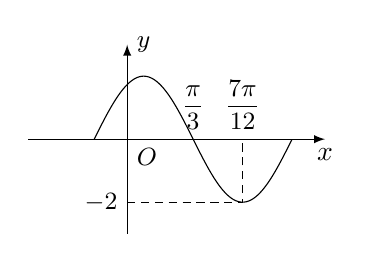
\begin{tikzpicture}[scale=0.8]
\coordinate[label=below right:\small $O$] (O) at(0,0);
\coordinate[label=above :\small $\dfrac{\pi}{3}$] (t1) at(pi/3,0);
\coordinate[label=above :\small $\dfrac{7\pi}{12}$] (t2) at(7*pi/12,0);
\draw[->,>=latex](-pi/2,0)--(pi,0)node[below](x) {$x$};
\draw[->,>=latex](0,-1.5)--(0,1.5)node[right](y) {\small $y$};
\draw [domain=-pi/6:5*pi/6,samples=1000] plot(\x,{sin((2*(\x)+pi/3) r)});
\draw[densely dashed](0,-1)--(7*pi/12,-1)--(7*pi/12,0);
\node[left](pi) at(0,-1) {\small $-2$};
\end{tikzpicture}
\end{center}
%\end{minipage}
%\hfill
%\begin{minipage}[b]{0.4\linewidth}
%\end{minipage}
\question 下列有关命题的说法正确的是\xx.
\fourch{命题“若~$x=y$~,则~$\sin x=\sin y$~”的逆否命题为真命题}{函数~$f(x)=\tan x$~的定义域为~$\{x\,|\,x\neq k\pi,k\in Z$~}
{命题“~$\exists x\in R$~使得~$x^2+x+1<0$~”的否定是:“~$\forall x\in R$~,均有~$x^2+x+1<0$~".}
{“$a=2$~”是“直线~$y=-ax+2$~与~$y=\dfrac{a}{x} x-1$~垂直”的必要不充分条件.}
\question 执行如图所示的程序框图,输出的$s$值为~\xx.
\twoch{$-3$}{$-\dfrac{1}{2}$}{$2$}{$\dfrac{1}{3}$}
\question 设函数~$y=x^3$~与~$y=\left(\dfrac{1}{2} \right)^{x-2}$~的图象的交点为~$(~x_0,y_0~)$~,则~$x_0$~所在的区间是\xx.
\twoch{$(0,1)$}{$(1,2)$}{$(2,3)$}{$(3,4)$}
\question 一个空间几何体的三视图如图,则该几何体的体积为\xx.

\twoch{$2\sqrt{3}$}{$2\sqrt{5}$}{$\dfrac{4\sqrt{3}}{3}$}{$\dfrac{5\sqrt{3}}{3}$}
\clearpage
\begin{figure*}[!htb] 
\begin{minipage}[t]{0.5\textwidth}%并排放两张图片,每张占页面的0.5,下同。  
\vspace{-1cm}
\centering  
% \includegraphics[scale=0.9]{liuchengtu.pdf}
\end{minipage}  
\begin{minipage}[t]{0.5\textwidth}  
\vspace{0cm}
\centering  
% \includegraphics[scale=0.9]{sanshitu.pdf}
\end{minipage}  
\end{figure*}
\vspace{-2cm}
%填空题
\tiankong
\question 已知向量~$\vec{a}=(3,1),\vec{b}=(1,3),\vec{c}=(k,7)$~,若~$(\vec{a}-\vec{c}) \parallel \vec{b}$~,则~$k=$~\mtk{}.
\question 等比数列~$\{a_n \}$~的公比~$q>0$~,已知~$a_2=1,a_{n+2}+a_{n+1}=6a_n$~,则~$\{a_n \}$~的前~$4$~项和~$S_4$~\mtk{}.
\question 设~$z=kx+y$~,其中实数~$x,y$~满足~$ \begin{cases}
x+y-2\geq 0,\\
x-2y+4\geq 0, \\
2x-y-4\leq 0,
\end{cases}$若~$z$~的最大值为~$12$~,则实数~$k=$~\mtk{}.
\question 设~$f(x)$~表示~$x+2$~与~$x^2+3x+2$~中的较大者,则~$f(x)$~的最小值为\mtk{}.
\question 设~$a\in R,f(x)=\cos (a\sin x-\cos x)+\sin ^2 x$~的定义域是~$\left[ \dfrac{\pi}{4},\dfrac{11}{24} \pi \right]~,f(\dfrac{\pi}{4})=\sqrt{3}$~.\\给出下列几个命题:\\
\ding{192}~$f(x)$~在~$x=\dfrac{\pi}{4}$~处取得最小值;\ding{193}~$\left[ \dfrac{5}{12} \pi,\dfrac{11}{24} \pi \right]$~是~$f(x)$~的一个单调递减区间;\\
\ding{194}~$f(x)$~的图象向左平移~$\dfrac{\pi}{12}$~个单位,将得到函数~$y=2\sin {2x}$~的图象;\\
\ding{195}使得~$f(x)$~取得最大值的点仅有一个~$x=\dfrac{\pi}{3}$~.\\
其中正确命题的序号是\mtk{}.(将你认为正确命题的序号都填上)
%解答题
\jianda
\question 在~$\triangle ABC$~中,角~$A,B,C$~的对边分别为~$a,b,c$~,已知~$A=\dfrac{\pi}{2}+C,\sin (A+C)=\dfrac{3}{5}$~.
\begin{parts}
\part 求~$\cos C$~的值;
\part 若~$a+c=3\sqrt{5}$~,求~$\triangle ABC$~的面积.
\end{parts}
\vspace{6cm}
\question 有甲乙两个班级进行数学考试,按照大于等于分为优秀,分以下为非优秀统计成绩后,得到如下的列联表.
\begin{center}
\begin{tabular}{|c|c|c|c|}
\hline
~~~~~~~{}~~~~~~~&~~~~~~~优秀~~~~~~~&~~~~~~~非优秀~~~~~~~&~~~~~~~总计~~~~~~~\\
\hline
~~~~~~~甲班~~~~~~~&~~~~~~~10~~~~~~~&~~~~~~~{}~~~~~~~&~~~~~~~{}~~~~~~~\\
\hline
~~~~~~~乙班~~~~~~~&~~~~~~~{}~~~~~~~&~~~~~~~30~~~~~~~&~~~~~~~{}~~~~~~~\\
\hline
~~~~~~~合计~~~~~~~&~~~~~~~{}~~~~~~~&~~~~~~~{}~~~~~~~&~~~~~~~105~~~~~~~\\
\hline
\end{tabular}
\end{center}
已知在全部~$105$~人中抽到随机抽取~$1$~人为优秀的概率为~$\dfrac{2}{7}$~.
\begin{parts}
\part 请完成上面的列联表; 
\part 根据列联表的数据,若按~$95 \%$~的可靠性要求,能否认为”成绩与班级有关系”;
\part 若按下面的方法从甲班优秀的学生抽取一人:把甲班优秀的~$10$~名学生从~$2$~到~$11$~进行编号,先后两次抛掷一枚均匀的骰子,出现的点数之和为被抽取人的序号.试求抽到~$6$~或~$11$~号的概率.
\end{parts}
下面临界值表仅参考:
\begin{tabular}{|c|c|c|c|c|c|c|c|}
\hline
$P(K^2\geq k_0)$&$0.15$&$0.10$&$0.05$&$0.025$&$0.010$&$0.005$&$0.001$\\
\hline
$k_0$&$2.072$&$2.706$&$3.841$&$5.024$&$6.635$&$7.879$&$10.828$\\
\hline
\end{tabular}\\
(参考公式:~$K^2=\dfrac{n(ad-bc)^2}{(a+b)(c+d)(a+c)(b+d)}$~,其中~$n=a+b+c+d$~)
\vspace{8cm}
\question 已知数列~$\{a_n \}$~是公差不为~$0$~的等差数列,~$a_1=2$~且~$a_2,a_3,a_4+1$~成等比数列.
\begin{parts}
\part 求数列~$\{a_n \}$~的通项公式;
\part 设~$b_n=\dfrac{2}{n\cdot (a_n+2)}$~,求数列~$\{b_n \}$~的前~$n$~项和~$S_n$~.
\end{parts}
\vspace{6cm}
\question 如图,在直三棱柱~$ABC--A_1B_1C_1$~中,~$AA_1=2,AB=AC=1,\angle BAC=90^{\circ}$~,点~$M$~是~$BC$~的中点,点~$N$~在侧棱~$CC_1$~上.
\begin{parts}
\part 求证:~$A_1C \parallel$~ 面~$AB_1M$~;
\part 当线段~$CN$~的长度为多少时,~$NM\perp AB_1$~.
\end{parts}
\begin{flushright}
\begin{tikzpicture}
\coordinate[label=below left:$B$](B) at (0,0);
\coordinate[label=below right:$C$](C) at (3,0);
\coordinate[label=left:$B_1$](B_1) at (0,3);
\coordinate[label=right:$C_1$](C_1) at (3,3);
\draw(B)--(C)--(C_1)--(B_1)--cycle;
\coordinate[label=above right:$A$](A) at (1.6,0.866);
\coordinate[label=above:$A_1$](A_1) at (1.6,3.866);
\coordinate[label=below:$M$](M) at ($(B)!0.5!(C)$);
\coordinate[label=right:$N$](N) at ($(C)!0.4!(C_1)$);
\draw(B_1)--(M)--(N)--(B_1);
\draw(B)--(A)--(C);
\draw(B_1)--(A_1)--(C_1);
\draw[dashed] (B)--(A_1)--(C) (B_1)--(A) (A)--(M) (A)--(N) (A)--(A_1);
\end{tikzpicture}
\end{flushright}
\vspace{1cm}
\question 已知~$E(2,2)$~是抛物线~$C:y^2=2px(p>0)$~上一点,经过点~$(2,0)$~的直线~$l$~与抛物线~$C$~交于~$A,B$~两点(不同于点~$E$~),直线~$EA,EB$~分别交直线~$x=-2$~于点~$M,N$~.
\begin{parts}
\part 求抛物线方程及其焦点坐标;
\part 已知~$O$~为原点,求证:~$\overrightarrow{OM}\cdot \overrightarrow{ON}=0$~
\end{parts}
\vspace{6cm}
\question 已知函数~$f(x)=x-a\ln x,g(x)=\dfrac{1+a}{x}(a\in R)$~.
\begin{parts}
\part 当~$a=1$~时,求曲线~$f(x)$~在~$x=1$~处的切线方程;
\part 设函数~$h(x)=f(x)-g(x)$~,求函数~$h(x)$~的单调区间.
\end{parts}
\end{questions}
\end{document}
